% !Mode:: "TeX:UTF-8"

\chapter{系统测试与分析}

本章主要是对已完成的魔方复原系统进行实验、测试以及与现有的魔方复原系统进行对比分析。得到以下实验结果:

\section{魔方块颜色识别实验}

在本实验中,将魔方随机打乱50次,每次获取48个魔方块的颜色,得到实验结果如下所示:

\noindent
\begin{minipage}{\textwidth}
	\vspace{1.0em}
	\begin{minipage}[t]{0.48\textwidth}
		\makeatletter\def\@captype{table}
		\caption{颜色识别实验结果}
		\label{tab:4-1}
		\vspace{1.5em}
		\begin{tabular}{cccc}
			\toprule
			颜色&识别正确率&颜色&识别正确率 \\
			\midrule
			白&100\%&红&99.5\%\\
			橙&98.3\%&蓝&100\%\\
			绿&100\%&黄&100\%\\
			\bottomrule
		\end{tabular}
	\end{minipage}
	\hfill
	\begin{minipage}[t]{0.48\textwidth}
		\makeatletter\def\@captype{table}
		\caption{颜色误识别次数表}
		\label{tab:4-2}
		\vspace{1.5em}
		\begin{tabular}{ccc}
			\toprule
			原颜色&误识别颜色&误识别次数\\
			\midrule
			红&白&2\\
			橙&红&5\\
			橙&白&2\\
			\bottomrule
		\end{tabular}
	\end{minipage}
\end{minipage}
\vspace{0.5em}

由上表~\ref{tab:4-1}~可知,在测试环境下,白色、蓝色、绿色、黄色的识别正确率均为100\%,但红色、橙色的识别正确率分别为99.5\%、98.3\%。由表~\ref{tab:4-2}~可以看出,在该实验中,有两次将红色误识别为白色,有五次将橙色误识别成红色,有两次将橙色误识别为白色。仔细观察颜色识别前后的图片后发现,有一部分原因是测试环境中的部分灯源直接照射到魔方块上导致魔方块反光,摄像头捕捉到的魔方块为反光后的白色,因此造成误识别。还有另外一部分原因是橙色与红色的色调分量有些接近,导致无法区分二者颜色。但考虑到系统颜色误识别的次数比较少,也允许系统存在一些偶然误差,因此总体上来看系统在魔方块颜色识别上的表现还是令人满意的。

\section{魔方复原算法对比分析}

本文对几种应用于现有魔方系统的解魔方算法进行实验分析,其中包括层先法~\cite{39}、CFOP法、角先法、Thistlethwaite算法以及Kociemba算法。后两种算法已经在本文3.3.2节与3.3.3节中详细介绍,此处便不赘述,下述是其他各个算法的简要介绍:

层先法的思路是以层为单位,逐层复原。先是在第一层拼成交叉十字形, 接着通过旋转使第二层的四个棱块归位,最后复原第三层。看似简单的思路每一层的旋转步骤却格外复杂,转动序列也较长,存在较多的冗余操作。

CFOP法是对层先法的改进,改进之处在于第一层到第二层、第二层到第三层的复原不需要进行转换,不需要进行多余的操作,但该方法并不能解决上述提到的冗余问题,仍存在旋转步骤多等问题。

角先法的思路与层先法类似,该方法并没有先将特定的某个面复原,而是先复原互不干扰的几个角块,最后根据特定的变换公式将整个魔方复原,复原的过程中虽然会破坏复原好的角块,但是并不会影响最后的复原结果。其复原的平均步骤数稍优于层先法,但与Kociemba算法仍存在较大差距。

针对上述五种魔方复原算法,本文对10组不同状态下的魔方进行复原步骤的计算与统计,得到平均值如下图所示:

\begin{figure}[H]
	\centering
	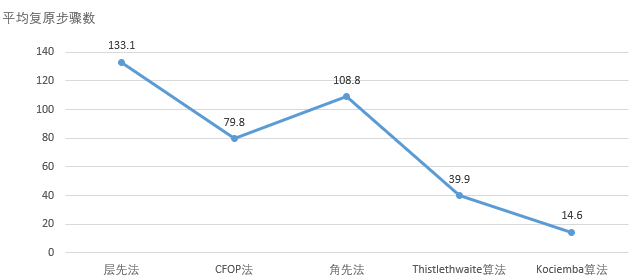
\includegraphics[width=\textwidth]{4-1}
	\caption{还原可行性效果图}\label{fig:4-1}
\end{figure}

由图4-1可以看出,在平均复原步骤数这个指标上,Koicemba算法具有明显优势。此外,在魔方复原系统的机械构造、整体框架相同的情况下,平均复原步骤数越少,其复原速度越快。因此,本论文选取Kociemba算法作为本系统的魔方复原算法可极大程度地提升魔方复原的速度。

\section{串并行复原实验}

本文对系统中的串行复原与并行复原进行十次对比实验,得到以下实验数据:

\begin{table}[H]
	\caption{串并行复原实验数据表}\label{tab:4-3}
	\vspace{0.5em}
	\begin{center}
		{\wuhao
			\begin{tabular}{cccc}
				\toprule
				实验编号 & 总步骤数	& 串行操作耗时(单位:秒)&并行操作耗时(单位:秒)\\
				\midrule
				1&13&1.52&1.28\\
				2&16&1.83&1.62\\
				3&14&1.46&1.44\\
				4&17&1.99&1.68\\
				5&13&1.41&1.30\\
				6&20&2.35&1.94\\
				7&15&1.70&1.63\\
				8&16&1.79&1.55\\
				9&20&2.16&2.03\\
				10&19&1.99&1.92\\
				\bottomrule
		\end{tabular}}
	\end{center}
	\vspace{-1.5em}
\end{table}

上表的每组数据中,当复原魔方的总步骤数相同时,并行操作消耗的时间总是比串行操作消耗的时间要少,将上述数据中每次实验的串行操作耗时与并行操作耗时除以复原步骤数即可得到复原单位步骤所消耗的时间,如下折线图所示。

\begin{figure}[H]
	\centering
	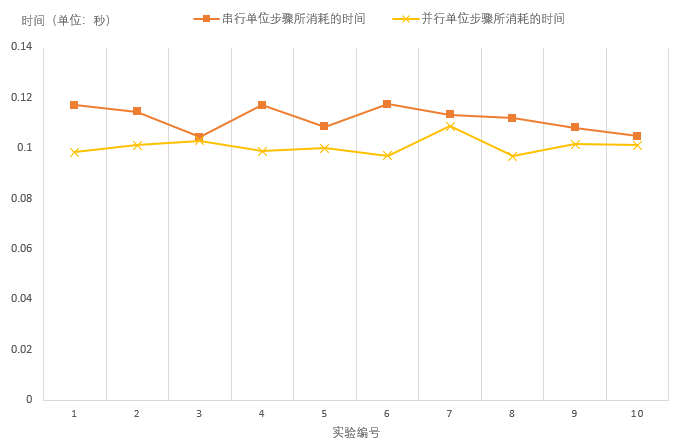
\includegraphics[width=\textwidth]{4-2}
	\caption{单位步骤耗时图}\label{fig:4-2}
\end{figure}

由上表~\ref{tab:4-3}~与上图~\ref{fig:4-2}~的数据可以得出,并行操作的复原速度总是优于串行操作,因为在并行操作过程中总能将其复原序列中互不干扰的旋转操作并行化,而单位旋转操作的耗时又相同,因此整体旋转操作数较少的方法,即并行操作,所耗费的时间也相对较少。

\section{本章小结}

本章从魔方块颜色识别、魔方复原算法与串并行复原三个方面对本系统进行对比实验。实验表明,本系统的魔方块颜色识别算法的识别正确率优于其他系统,并且魔方复原算法与并行还原优化算法均能在一定程度上有效提高魔方复原的速度,实现魔方的快速还原。